%************************************************
\chapter{Konzept}\label{ch:concept}
%************************************************
%
Beim klassischen Client Server Modell muss sich jeder Client Ressourcen über das WAN laden. Abbildung \ref{fig:school} zeigt den typischen Aufbau eines solchen Netzwerks. Sind die geladenen Ressourcen groß kann die WAN Anbindung zu einem Flaschenhals werden. Durch die dadurch resultierenden langen Ladezeiten kann es zu einer starken Einschränkung des Nutzererlebnisses und der Nutzerzufriedenheit kommen.(\emph{\color{red} studie einfügen })

\begin{figure}[!h]
	\centering
	\includegraphics[width=0.8\textwidth]{figures/school}
	\caption[A Figure Short-Title]{Lebenszyklus eines Service Workers\footnote{https://developers.google.com/web/fundamentals/primers/service-workers/}}
	\label{fig:school}
\end{figure}

In den Betrachteten Anwendungsfällen besteht eine hohe zeitlich und inhaltliche Lokalität der Daten. Dies kann genutzt werden um die benötigte Bandbreite zu reduzieren. Dazu soll im Folgenden eine interne Verteilung mittels eines hybriden \pTp Ansatzes untersucht werden. Abbildung \ref{fig:mesh} zeigt exemplarisch den Aufbau eines solchen Netzwerkes. Anstatt das jeder Client sich die Ressource von einem externen Server lädt, lädt nur noch ein Nutzer je Subnetz die Resource über das WAN. Dieser verteilt die Resource dann im internen Netzwerk an andere Clients die diese dann ebenfalls wieder bereitstellen.

Benötigt ein Client eine Resource versucht er zuerst die Resource über sein \pTp Mesh zu laden. Ist dies nicht möglich lädt er sie über einen externen Server. Hat ein Peer eine Resource geladen speichert er sie zwischen und stellt sie für andere Clients bereit.

\begin{figure}[!h]
	\centering
	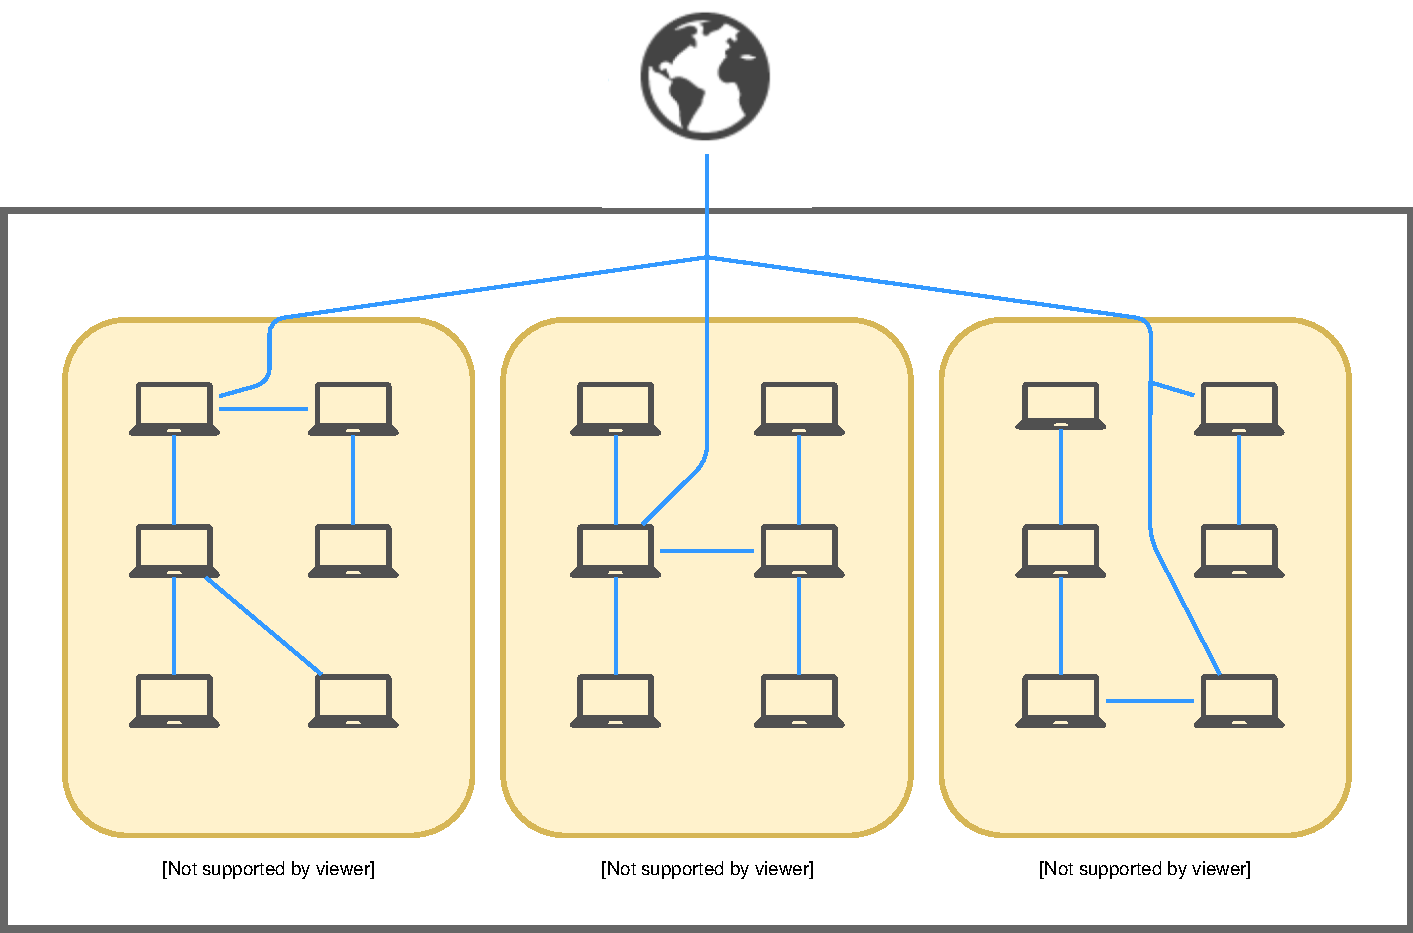
\includegraphics[width=0.8\textwidth]{figures/mesh}
	\caption[A Figure Short-Title]{Lebenszyklus eines Service Workers\footnote{https://developers.google.com/web/fundamentals/primers/service-workers/}}
	\label{fig:mesh}
\end{figure}

Da sowohl im Kontext der Schule als auch bei Unternehmen kein Wissen im Bereich der Computer Administration vorausgesetzt werden soll, soll ein Ansatz gewählt werden der keine Installation auf Seiten der Nutzer benötigt. Das Nutzererlebnis sollte nicht negativ beeinflusst werden. 

% herausstellen das ein plugin entwickelt wird das eingebunden werden kann


% schon geschrieben:
%Genereller Architektur Ansatz
% interne verteilung in subnetzen vs wan verbindung
% Klassische Server architekur mit client und server beschreiben + bild
% p2p mit bild zeigen netzarchitektur
% kommunikation zwischen peer anhand von vereinfachter architektur beschreiben
%	bild peer to peer zwischen browsern ohne service worker
%	peer to peer zwischen browsern
% hybrid p2p CDN ansatz
% keine installation auf clientseite
% domainen wissen soll genutzt werden um clients zu verbinden
% 
%
%
%


%bild schule wie in blockpost?
%
%
%%

% "hybrid p2p cdn"
%konfiguration von subnetzen?


\section{Mesh Zuordnung - Verbinden von Peers}

% voll vermaschtes netz
% mit bild
% Nutzung des anwendungswissens
% ip subnetz plus gleicher Kurs/stream


\section{Objekt Zuordnung - finden von Ressourcen}

Um das \pTp Netzwerk als \cdn Nutzbar zu machen ist es wichtig das ein Peer in der Lage ist herauszufinden wer welche resource bereitstellt. Dazu lassen sich verschiedene Ansätze verfolgen. 

server hält liste vor --> kommunikation mit server nötig. \study

peer fragt im Netzwerk an --> mehr kommunikation wenn in zeitkritischem moment \study

peer halten liste von requests aktuell. Kommunikationsoverhead in zeitunkritischem moment \study
%	 peer weiß immer bei wer welche resource hat

% evtl diskussion verschiedener methoden 
%   server hält liste vor --> kommunikation mit server nötig
% peer fragt im Netzwerk an --> mehr kommunikation wenn in zeitkritischem moment
% peer halten liste von requests aktuell
%    kommunikationsoverhead in zeitunkritischem moment
%	 peer weiß immer bei wer welche resource hat
% am Anfang wird die zuordnung von einem peer an den neuen geschickt


\subsection{Subnetzerkennung}
\subsection{ Struktur von IP Adressen}
eher Konzept


\section{Wiederverwendbarkeit}
%Plug and play
%Konfigurierbarkeit
%einfaches einbinden in existierende anwendungen über npm
%javascript modul
%support von eigenen oder öffentlichen stun servern
%%Plug and play
\section{Open Source}
%was ist open source
%bereitstellung für die öffentlichkeit
%
